\documentclass[a4paper,11pt]{jsarticle}
\usepackage{amsmath,amssymb}
\usepackage{bm}
\usepackage[dvipdfmx]{graphicx}
\usepackage{here}%figureにoption[H]を付けるとその場に表示
\usepackage{listings,jlisting}%コードを載せる
\usepackage{multicol}%部分的に二段組にする

%テキストの表示領域の調節
\setlength{\textwidth}{\paperwidth}
\addtolength{\textwidth}{-40truemm}
\setlength{\textheight}{\paperheight}
\addtolength{\textheight}{-45truemm}

%余白の調節
\setlength{\topmargin}{-10.4truemm}
\setlength{\evensidemargin}{-5.4truemm}
\setlength{\oddsidemargin}{-5.4truemm}
\setlength{\headheight}{17pt}
\setlength{\headsep}{10mm}
\addtolength{\headsep}{-17pt}
\setlength{\footskip}{5mm}

\begin{document}

\section{実験の目的}
簡単なロボットによる作業の演習を通してロボット言語によるプログラムの作成及びロボットの操作法を習得するとともに,
ロボットのメカニズム, 運動学, 制御法などに関する一般的な理解を深める.

\section{実験システム}%ロボット及びバレタイズに必要な周辺装置
\subsection{ロボットアーム}

本実験では,  三菱電機製のロボット RV-2SDを使用した.
本ロボットは, 産業用ロボットを教育用途に小型化した製品である(図\ref{ロボット}).
\begin{figure}[H]
  \begin{center}
    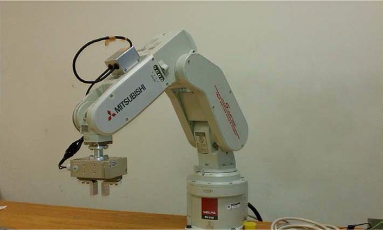
\includegraphics[width = 8cm]{画像/ロボットアーム.png}
    \caption{ロボットアーム RV-2SD}
    \label{ロボット}
  \end{center}
\end{figure}

このロボットは「垂直多関節ロボット」あるいは「6軸多関節ロボット」と呼ばれる機構をしており, 6つの回転関節
を持つ. 各関節は接地部分に近い順に第1, 第2 $\cdots$ 第6関節と呼ばれる他, それぞれに固有の呼称も存在する. 以下では
第一関節から順に説明していく. \par
第1関節, つまりロボットの接地部分から一つ目の関節は, ウエスト関節とも呼ばれる(図\ref{ウエスト関節}).
この関節は人間の腰関節に相当する.
\begin{figure}[H]
  \begin{center}
    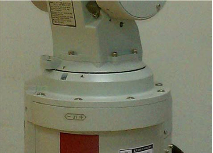
\includegraphics[width = 7cm]{画像/ウエスト関節.png}
    \caption{ウエスト関節(第1関節)}
    \label{ウエスト関節}
  \end{center}
\end{figure}

\newpage
第2関節, つまり接地部分から二つ目の関節は, ショルダー関節とも呼ばれる(図\ref{ショルダー関節}). 人間の肩関節に相当する.
\begin{figure}[H]
  \begin{center}
    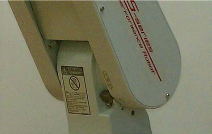
\includegraphics[width = 7cm]{画像/ショルダー関節.png}
    \caption{ショルダー関節(第2関節)}
    \label{ショルダー関節}
  \end{center}
\end{figure}

第3関節はエルボー関節とも呼ばれる(図\ref{エルボー関節}). 人間の肘関節に相当する.
\begin{figure}[H]
  \begin{center}
    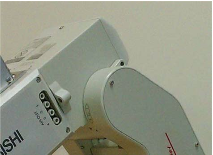
\includegraphics[width = 7cm]{画像/エルボー関節.png}
    \caption{エルボー関節(第3関節)}
    \label{エルボー関節}
  \end{center}
\end{figure}

第4関節はツイスト関節とも呼ばれる(図\ref{ツイスト関節}). 人間の肘の捻りに相当する運動を行う.
\begin{figure}[H]
  \begin{center}
    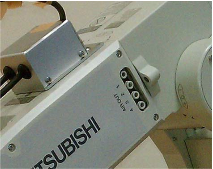
\includegraphics[width = 7cm]{画像/ツイスト関節.png}
    \caption{ツイスト関節(第4関節)}
    \label{ツイスト関節}
  \end{center}
\end{figure}

第5関節はリストピッチ関節と呼ばれる(図\ref{リストピッチ関節}). 人間の手首関節のピッチ運動に相当する運動を行う.
\begin{figure}[H]
  \begin{center}
    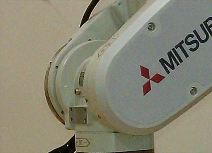
\includegraphics[width = 7cm]{画像/リストピッチ関節.png}
    \caption{リストピッチ関節(第5関節)}
    \label{リストピッチ関節}
  \end{center}
\end{figure}

第6関節はリストロール関節と呼ばれる(図\ref{リストロール関節}). 人間の手首関節の回転方向に相当する運動を行う.
\begin{figure}[H]
  \begin{center}
    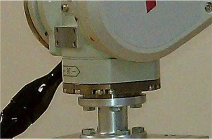
\includegraphics[width = 7cm]{画像/リストロール関節.png}
    \caption{リストロール関節(第6関節)}
    \label{リストロール関節}
  \end{center}
\end{figure}

以上の6関節の回転を組み合わせることで, ロボットアームの動作を行っている.
\par
各関節の駆動にはACサーボモータが使用されている.ACサーボモータとDCサーボモータの構造を図\ref{サーボモータの構造}に示す.
ACサーボモータは入力信号に交流電流を使用するため,制御が難しいが,DCサーボモータと違いブラシレスでメンテナンスフリー
であることから,ロボットアームなどに採用される場面が増えてきている.
\begin{figure}[H]
  \begin{center}
    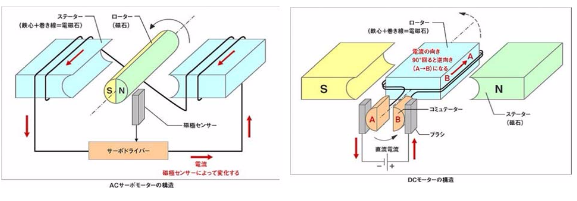
\includegraphics[width = 10cm]{画像/サーボモータの構造.png}
    \caption{サーボモータの構造}
    \label{サーボモータの構造}
  \end{center}
\end{figure}

\par
関節角度を測定するために,各関節に絶対位置エンコーダ(アブソリュートエンコーダ)が搭載されている.絶対位置エンコーダ
は相対位置エンコーダ(通常のエンコーダ)と比較すると高価であるが,原点出しが不要であるため,作業開始時の準備段階を減らすことができる.
また,関節駆動に対して、ロータリーエンコーダによってフィードバック制御を行なっている.各関節にはブレーキがかかるようになっており,
電源を切ると関節が動かないようになっている.
\par
このような大き機械を動かす場合,モータで直接駆動しようとすると非常に大きなものを採用しなければ,
必要となるトルクを得ることは難しい.そのため,減速機を用いるのが一般的である.特にロボットのような空間的制約
のある危機に対して多く利用されている減速機がハーモニックドライブである(図\ref{ハーモニックドライブ}).
ハーモニックドライブは歯車を利用した減速機よりも少ないスペースで高減速比を実現することが可能である.
\begin{figure}[H]
  \begin{center}
    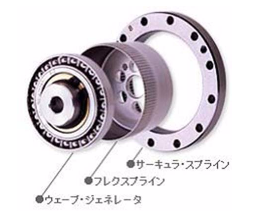
\includegraphics[width = 8cm]{画像/ハーモニックドライブ.png}
    \caption{ハーモニックドライブ}
    \label{ハーモニックドライブ}
  \end{center}
\end{figure}

\subsection{電動ハンド}
ロボットアームに TAIYO 製の電動ハンド ESG1-FT-2840(図\ref{電動ハンド})を装着して対象物の把握を行った.
このハンドは2爪の平行グリッパによって把持を行い, グリッパはモータとボールネジを利用して駆動している.
また, ハンドには絶対一エンコーダではなく相対位置エンコーダが搭載されているため, ハンドはアームと異なり, 電源を入れるたびに原点出しの準備動作が必要となる.

\begin{figure}[H]
  \begin{center}
    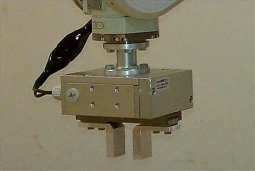
\includegraphics[width = 8cm]{画像/電動ハンド.png}
    \caption{電動ハンド ESG1-FT-2840}
    \label{電動ハンド}
  \end{center}
\end{figure}

\subsection{コントローラ}
コントローラはロボットの制御に使用するプログラムを実行し, 制御時に必要な各種計算(運動学計算や逆運動学計算など)
を行う装置である(図\ref{コントローラ}). 本実験で利用したコントローラは TCP/IP 通信でPCに接続されており,
PCとの間でプログラムの送受信を行い, プログラムの選択・実行などをPC側から行うことができる.

\begin{figure}[H]
  \begin{center}
    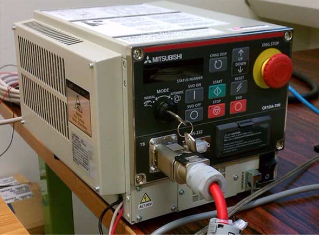
\includegraphics[width = 10cm]{画像/コントローラ.png}
    \caption{コントローラ}
    \label{コントローラ}
  \end{center}
\end{figure}

\subsection{ティーチングボックス}
ティーチングボックス(ティーチングペンダント)は, ロボットアームに座標を表示するための装置である(図\ref{ティーチングボックス}).
本実験で使用したものは高機能で, 教示の他に電動ハンドの制御や外部入力のデバッグ, プログラムの編集や実行も可能である.

\begin{figure}[H]
  \begin{center}
    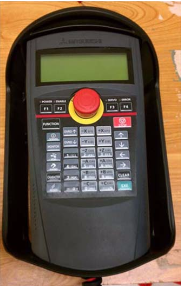
\includegraphics[width = 5cm]{画像/ティーチングボックス.png}
    \caption{ティーチングボックス}
    \label{ティーチングボックス}
  \end{center}
\end{figure}

\subsection{パレタイズ}
パレタイズとは等間隔に整列された容器(パレット)に対象となる物体(ワーク)を指定した通りの順番で,
適当な位置に移動させ,置いていくという作業のことをいう.日常生活で触れるものでは卵のパックなどがパレットの代表例としてあげられる.
このような製品は当然,入っているべき個数が入っているべき場所に収まっていることが重要となる.
よって,バレタイズ作業を正確に行えるということは製品を製造する場面で重要な要素であると言える.
\par
今回の実験で使用したパレットを図\ref{パレット}に示す.
\begin{figure}[H]
  \begin{center}
    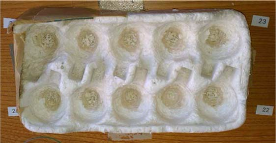
\includegraphics[width = 10cm]{画像/パレット.png}
    \caption{パレット}
    \label{パレット}
  \end{center}
\end{figure}

\subsection{オートパーツフィーダー}
オートパーツフィーダー(自動部品供給器)とは,ワークを同じ場所に送り続けることで,教示座標の点数を減らすことができるようにする装置のことである.
今回の実験に使用したものを図\ref{オートパーツフィーダー}に示す.
\begin{figure}[H]
  \begin{center}
    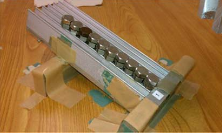
\includegraphics[width = 8cm]{画像/オートパーツフィーダー.png}
    \caption{オートパーツフィーダー}
    \label{オートパーツフィーダー}
  \end{center}
\end{figure}

\subsection{スイッチ}
今回はワークの把持ができているか確認するためのデバッグを,図\ref{スイッチ}に示すスイッチを利用することで行なった.
\begin{figure}[H]
  \begin{center}
    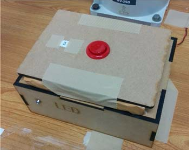
\includegraphics[width = 8cm]{画像/スイッチ.png}
    \caption{スイッチ}
    \label{スイッチ}
  \end{center}
\end{figure}


\section{実験内容と手順}
本実験は以下のような流れでロボットアームに作業を行わせた(図\ref{作業の流れ}).
\begin{figure}[H]
  \begin{center}
    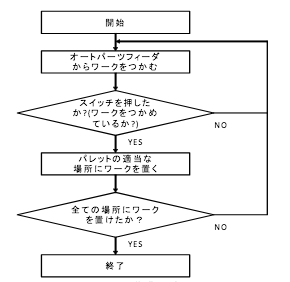
\includegraphics[width = 7cm]{画像/作業の流れ.png}
    \caption{ロボットアームの作業の流れ}
    \label{作業の流れ}
  \end{center}
\end{figure}

\subsection{教示}
ロボットにパレタイズ作業を行わせるために,ティーチングボックス(TB)を用いて,各ポジションの教示を行わなければいけない.
\par
本実験で使用する装置は,プログラムごとにポジションの名前を設定し,各ポジションに対して教示を行う.
よって,教示を行う前にプログラムを用意し,TBでそのプログラムを開く必要がある.今回の実験では,事前に用意した
基本的なパレタイズ作業を行うプログラム"sample2.prg"に対して教示を行なった.

\subsubsection{教示の位置}
ポジション1(P1):ボルトを掴む位置
\begin{enumerate}
  \item TBでボルトを掴める位置までロボットのハンドを動かす.その時,ボルトを引き上げる時にアームの姿勢を考慮して,位置を決めた.
  \item ハンドを開いたままポジションを教示する.
  \item ハンドを閉じ,ボルトを掴む.
  \item 持ち上げる.
\end{enumerate}
ポジション3(P3):スイッチを押す位置
\begin{enumerate}
  \item ボルトを掴んだ状態で,ボタンスイッチを押せるような位置を決めた.ボタンスイッチが押されると
  LEDが点灯されるので,それを確認しながら行なった.
  \item ポジションを記憶させる.
  \item ボルトを上に回避させる.
\end{enumerate}
ポジション2:ボルトを落とす位置
\begin{enumerate}
  \item パレットにある10個の穴の位置をロボットに教えるためには,4隅の上でボルトを落とせる位置(ポジション番号 20,21,22,23)
  を教示すれば良い.教示する際,ハンドの高さはパレットの淵よりも少し高くした.
\end{enumerate}

\subsubsection{パレタイズ例題}
教示作業が終了したのち,例として図\ref{パレタイズ例}のような順序でパレタイズ作業を行なわせた.
\begin{figure}[H]
  \begin{center}
    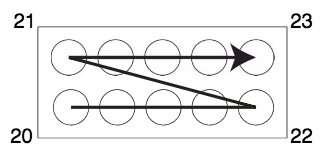
\includegraphics[width = 10cm]{画像/パレタイズ順序例.png}
    \caption{パレタイズ順序:例題}
    \label{パレタイズ例}
  \end{center}
\end{figure}

\section{演習課題}
パレタイズ例題に使用したプログラムを改良して,図\ref{パレタイズ演習}の順序でパレタイズ作業を行うプログラムを作成し,
実際にロボット制御用コンピュータでプログラムを実行させた.

\begin{figure}[H]
  \begin{center}
    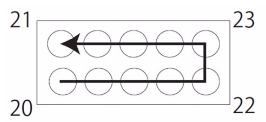
\includegraphics[width = 10cm]{画像/パターン1.png}
    \caption{パレタイズ順序:演習}
    \label{パレタイズ演習}
  \end{center}
\end{figure}

以下に改良プログラムのコードと各行に対する説明を示す.
\newpage
\begin{multicols}{2}
  \begin{lstlisting}[basicstyle=\ttfamily\footnotesize]
    1 Spd 20
    2 If M_EHOrg=0 Then  
    3    EHOrg 1
    4    Wait M_EHOrg=1
    5 EndIf
    6 For MI=0 To 1
    7    For MJ=0 To 4
    8      If MI = 0 Then
    9         PTemp=P20
    10        PTemp=PTemp + PV*MJ
    11     Else
    12        PTemp=P23
    13        PTemp=PTemp - PV*MJ
    14     Endif
    15     *LBL1 Mov P1, -30
    16     EHOpen 1, 50, 30
    17     Wait M_EHBusy=0
    18     Mvs P1
    19     EHClose 1, 50, 30
    20     Wait M_EHBusy=0
    21     Mvs P1, -15
    22     Mov P1, -70
    23     Mov P3, -20
    24     Def Act 1, M_In(31)=1 GoTo *LBL2
    25     Act 1=1
    26     Mvs P3
    27     Act 1=0
    28     Mvs P3, -20
    29     Mov PErr
    30     EHOpen 1, 50, 30
    31     Wait M_EHBusy=0
    32     GoTo *LBL1
    33     *LBL2  Act 1 = 0
    34     Mvs P3, -20
    35     Mov PTemp, -90
    36     Mov PTemp, -10
    37     EHOpen 1, 30, 30
    38     Wait M_EHBusy=0
    39     Mov PTemp, -50
    40    Next MJ
    41  Next MI
    42 End
    PTemp=(+424.52,-31.92,+172.64,-171.43,-12.49,-94.16,+0.00,+0.00)(7,0)
    P20=(+403.76,+138.90,+166.76,+175.18,-1.73,-96.51,+0.00,+0.00)(7,0)
    PV=(+0.00,-48.26,+0.00,+0.00,+0.00,+0.00,+0.00,+0.00)(0,0)
    PW=(+46.12,+0.00,+0.00,+0.00,+0.00,+0.00,+0.00,+0.00)(0,0)
    P1=(+365.96,-226.66,+156.70,-165.67,+4.82,-167.50,+0.00,+0.00)(7,0)
    P3=(+260.04,+25.14,+248.15,+179.30,-1.25,-96.72,+0.00,+0.00)(7,0)
    PErr=(+460.54,-133.35,+184.36,+177.63,-4.42,-134.98)(7,0)
    P0=(+375.14,-11.15,+299.92,-179.07,-4.90,-166.26)(7,0)
    P21=(+450.71,+141.59,+169.03,+174.36,-0.79,-84.77,+0.00,+0.00)(7,0)
    P22=(+408.24,-45.75,+166.76,+175.19,-1.72,-96.51,+0.00,+0.00)(7,0)
    P23=(+450.46,-47.81,+169.03,+174.36,-0.80,-84.82,+0.00,+0.00)(7,0)
1 速度を20に設定
2 ハンドの原点復帰が未完了ならば
3 ハンド1を原点復帰
4 ハンド1の原点復帰完了待ち
5 If文処理終了
6 数値変数MIを0から1まで+1ずつカウント
7 数値変数MJを0から4まで+1ずつカウント
8 MIが0ならば
9 数値変数PTempにP20を代入
10 PTempにPV*MJを足して更新
11 MIが0でなければ
12 PTempにP23を代入
13 PTempからPV*MJを引いて更新
14 If文処理終了
15 P1の上空30mmへ関節補間移動(*LBL1)
16 ハンド1を50%の速度と30%の力で開く
17 ハンド1の動作完了待ち
18 P1に直線補間移動
19 ハンド1を50%の速度と30%の力で開く
20 ハンド1の動作完了待ち
21 P1の上空15mmに直線補間移動
22 P1の上空70mmに関節補間移動
23 P3の上空20mmに関節補間移動
24 入力信号31が1になると*LBL2にジャンプを定義(Act1)
25 処理Act1の割り込みを許可
26 P3に直線補間移動
27 処理Act1の割り込みを禁止
28 P3の上空20mmに直線補間移動
29 PErrに関節補間移動
30 ハンド1を50%の速度と30%の力で開く
31 ハンド1の動作完了待ち
32 *LBL1(15行目)にジャンプ
33 処理Act1の割り込みを許可(*LBL2)
34 P3の上空20mmに直線補間移動
35 PTempの上空90mmに関節補間移動
36 Ptempの上空10mmに関節補間移動
37 ハンド1を30%の速度と30%の力で開く
38 ハンド1の動作完了待ち
39 PTempの上空50mmに関節補間移動
40 For MJ=0 To 4 (7行目)に戻る
41 For MI=0 To 1 (6行目)に戻る
42 プログラム終了










.
  \end{lstlisting}%ここを変えると崩れてしまうよ
\end{multicols}

\section{課題}

\subsection{順運動学では各関節の状態からロボットの手先の位置・姿勢が一位な解として求まるのに対し,
逆運動学では目的とするロボットの手先位置・姿勢から各関節の状態が一意に定まらないことをわかりやすく説明する.}
順運動学では一つの目標座標に対して各関節から追っていくため一意に定まるが,
逆運動学では目標座標に対して複数のロボットの状態が考えられる

図\ref{アーム}のような2自由度のロボットアームを考える. $x_2$と$y_2$が定まっている場合を順運動学と逆運動学それぞれについて解く.

\begin{figure}[H]
  \begin{center}
    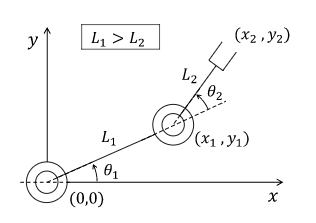
\includegraphics[width = 10cm]{画像/2自由度ロボットアーム.png}
    \caption{2自由度のロボットアーム}
    \label{アーム}
  \end{center}
\end{figure}

\subsubsection{順運動学}
一つ目のリンクの座標は次のようになる.
\begin{align}
  x_1=L_1\cos{\theta_1}\\
  y_1=L_1\sin{\theta_1}
\end{align}

二つ目のリンクの座標,つまり手先の位置$(x,y)$は次のようになる.

\begin{align}
  x_2&=x_1+L_2\cos{\theta_1 + \theta_2 }\\
     &=L_1\cos\theta_1+L_2\cos\left(\theta_1+\theta_2\right)
\end{align}

\begin{align}
  y_2&=y_1+L_2\sin\left(\theta_1+\theta_2\right)\\
     &=L_1\sin\theta_1+L_2\sin\left(\theta_1+\theta_2\right)
\end{align}

つまり, $\theta_1$と$\theta_2$が決まれば一意な$(x,y)$が得られる.
以上より,順運動学では各関節の状態からロボットの手先の位置・姿勢が一意な解として求まる.

\subsubsection{逆運動学}
手先位置$(x,y)$に対して,逆運動学では以下のような2つの解が求められる.
よって, 逆運動学では目的とするロボットの手先位置・姿勢から各関節の状態が位置に定まらない.
\begin{figure}[H]
  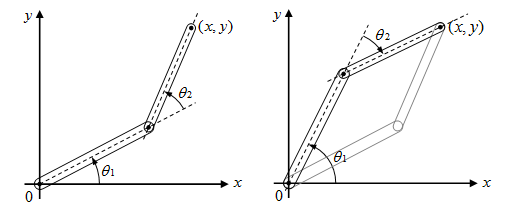
\includegraphics{画像/逆運動学.png}
  \caption{逆運動学により求められる2解}
  \label{逆運動学}
\end{figure}




\subsection{直接補間動作の場合, ロボットの始点座標と終点座標の与え方によっては,
ロボットが実行可能な経路を生成できなくなる場合がある. この実例を図\ref{アーム}のような2自由度のロボットアームを想定して1つ示す.}
図\ref{アーム}のロボットアームを例にとる.アームは$L_1>L_2$であることから, $L_1-L_2$を半径とする円の領域にはハンドが侵入できない.
そこで図\ref{直接補間}のように始点Aと終点Bを設定する. ハンドはA点からB点へ点線の経路に沿って直線的に移動しようとするが,
$L_1-L_2$を半径とする円からなる不可侵領域(色付けされた領域)を通ってしまうため,ロボットが実行可能な経路を生成できなくなってしまう.

\begin{figure}[H]
  \begin{center}
    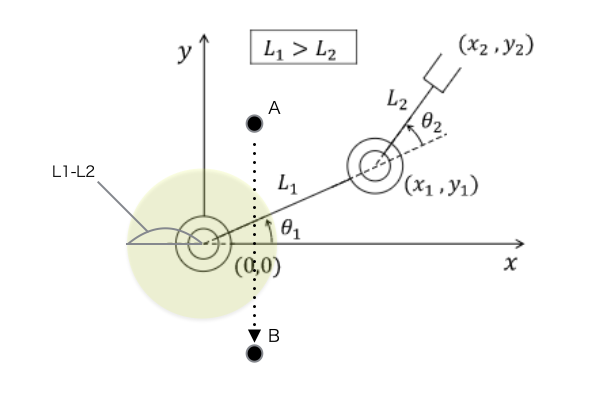
\includegraphics[width = 10cm]{画像/直接補間.png}
    \caption{直接補間移動が不能な例}
    \label{直接補間}
  \end{center}
\end{figure}

\subsection{ロボットの機構と制御法に関する基本事項}
ロボットは複数のリンクまたは節と呼ばれる剛体を連結して構成される.また連結の際,リンクが互いに相対的な運動を妨げない
ように,軸や軸受などを組み合わせて連結する.このように相対的に運動可能となるように結合されている部分をジョイント
,対偶などと呼ぶ.ジョイントは,リンクとリンクの間にアクチュエータを設置し,能動的に運動するものと,軸と軸受などにより
複数のリンクを連結し,リンクの運動に応じて受動的に運動するものがある.またロボットのジョイントには回転運動を行う回転ジョイント,
直進運動を行う直進ジョイントがある.以上で述べたジョイントやリンクを組み合わせてロボットの形式を決定する.
\par
ロボットの特徴はジョイントの種類によって大きく左右される(表\ref{ジョイント表}).

\begin{table}[H]
	\caption{ジョイントによるロボットの特徴}
	\label{ジョイント表}
	\begin{center}
		\begin{tabular}{c|c|c|c|c|c}\hline
		   & 剛性 & 制御 & 占有空間 & 作業領域 & 保守 \\ \hline
			回転ジョイント & 劣 & 劣 & 優 & 優 & 優\\ \hline
			直進ジョイント & 優 & 優 & 劣 & 劣 & 劣 \\ \hline
	   \end{tabular}
\end{center}
\end{table}

直進ジョイントを用いたメカニズムに作用する負荷は引張・圧縮であることが多く,回転ジョイントでは曲げであることが多い.
一般に、機械材料は引張・圧縮負荷に対する変形を生じにくいが,曲げに対しては大きな変形を生じやすい.そのため,
直進ジョイントを用いたロボットは剛性が高い場合が多い.また,直線ジョイントでは入出力関係が線形となり, 制御が容易であるが,
回転ジョイントでは入出力関係が三角関数などで表される非線形関係となるため,制御は複雑となる.
\par
ロボットが出力部をどの程度自由に動かせるかは,組み合わされるジョイント,リンクの構成によりほぼ決定される.
このようなロボットの運動の自由さを表すう数値として自由度が用いられる.自由度は一般に,ある物体の運動を表すために
必要な,独立した変数の数を表す.ロボットの運動は複数のジョイントがそれぞれ回転,直進することにより創成される.
しかし,ロボットの作業や制御を検討するときに対象となるのは,出力点または出力リンクすなわち出力部の運動である.
したがって,ロボットの自由度は出力部の運動を表す独立した変数の数で表される.その出力部は,ロボットに用いられる
能動ジョイントで運動させられるので,通常は,用いる能動ジョイント,言い換えればアクチュエータの数と自由度は一致する.

\subsubsection{今回の実験またはロボットに関する感想}
今回の実験ではロボットの仕組みと制御の基礎から学び,実際にロボットを動かし,教示したのちに動かし,また目標とする
動きをさせるためにプログラムを書き換え,実行させて動かす一連の流れを実験した.ロボットの力学の授業で学んだ事項
などが実際にどのように使われて,どのようなところを机上の知識に付け加えなければいけないのかがわかり,今まで学んだことへの
理解が一層深まったと共に今後のモチベーションにもつながる実験であった.また同様に運動学の理解など勉強が不十分であったと感じさせられる
部分もあり大変身にしみた.この実験を通して簡単な制御を行なったが,ボルトを持ち上げて順番に入れていくという簡単な動作一つでも
少し手こずってしまう場面などもあり,プログラミング的思考能力もより一層高めていかなければならないと感じた.現代ではほとんどのモノが
オートメーション化されており,産業用ロボットが世界を作っている.加えて, AIの発達により,単純ロボットのみならず複雑な動きを行うロボットが
これから街にも溢れ,社会においても重要な責務を担っていくと考えられるので,そうなったときにしっかりと可動できるロボットを作れる能力を持った
人材にならなければならないと今まで以上に感じた.


\end{document}
